\documentclass[aspectratio=169,11pt]{beamer}
\usetheme{default}
\setbeamertemplate{navigation symbols}{}
\setbeamertemplate{footline}{%
  \hfill\insertframenumber/\inserttotalframenumber\hspace*{4pt}\vspace{2pt}%
}
\usepackage{lmodern}
\usepackage[most]{tcolorbox}
\usepackage{listings}
\usepackage{tikz}
\usetikzlibrary{arrows.meta,positioning,shapes.geometric,fit,backgrounds}
\usepackage{booktabs}
\usepackage{hyperref}

\definecolor{lcgreen}{HTML}{2E7D32}
\definecolor{lcblue}{HTML}{1565C0}
\definecolor{lcorange}{HTML}{EF6C00}
\definecolor{lcred}{HTML}{C62828}
\definecolor{codebg}{HTML}{F5F5F5}
\definecolor{docgray}{gray}{0.55}

\newtcolorbox{conceptbox}[1][]{colback=yellow!20,colframe=yellow!60!black,title=#1,fonttitle=\bfseries}
\newtcolorbox{warningbox}[1][]{colback=red!15,colframe=red!60!black,title=#1,fonttitle=\bfseries}
\newtcolorbox{tipbox}[1][]{colback=green!10,colframe=green!50!black,title=#1,fonttitle=\bfseries}
\newtcolorbox{codebox}[1][]{colback=blue!10,colframe=blue!40!black,title=#1,fonttitle=\bfseries}

\lstset{
  basicstyle=\ttfamily\tiny,
  backgroundcolor=\color{codebg},
  breaklines=true,
  frame=single,
  rulecolor=\color{blue!40!black},
  keywordstyle=\color{lcblue}\bfseries,
  stringstyle=\color{lcgreen},
  commentstyle=\color{docgray}\itshape,
  language=Python,
  showstringspaces=false,
  tabsize=2,
  xleftmargin=2pt,
  xrightmargin=2pt,
}

\newcommand{\docref}[1]{{\scriptsize\color{docgray}[Docs: #1]}}

\title{LangChain Section 13: Putting It All Together}
\subtitle{Building a Production RAG Chatbot with Agent Capabilities}
\author{LangChain v1.2.x (March 2026)}
\date{}

\begin{document}

% ============================================================================
% SLIDE 1: Title
% ============================================================================
\begin{frame}
  \titlepage
  \begin{center}
    {\small A step-by-step guide to building a realistic, production-ready RAG system with agents, memory, and streaming.}
  \end{center}
\end{frame}

% ============================================================================
% SLIDE 2: Project Overview
% ============================================================================
\begin{frame}
  \frametitle{Project: Production RAG Chatbot with Agent Capabilities}

  \begin{columns}[T]
    \column{0.5\textwidth}
    \textbf{What we're building:}
    \begin{itemize}
      \item Intelligent chatbot answering questions about documents
      \item RAG for contextual, factual responses
      \item Agent with external tools (web search, calculator)
      \item Memory across conversation sessions
      \item Real-time streaming responses
      \item Full observability with LangSmith
      \item REST API for easy integration
    \end{itemize}

    \column{0.5\textwidth}
    \textbf{Technology stack:}
    \begin{itemize}
      \item LangChain --- orchestration
      \item LangGraph --- agentic workflows
      \item OpenAI API --- LLM (GPT-4)
      \item Pinecone --- vector database
      \item FastAPI --- REST API
      \item SQLite --- memory
      \item LangSmith --- tracing
    \end{itemize}
  \end{columns}
\end{frame}

% ============================================================================
% SLIDE 3: System Architecture
% ============================================================================
\begin{frame}
  \frametitle{System Architecture}

  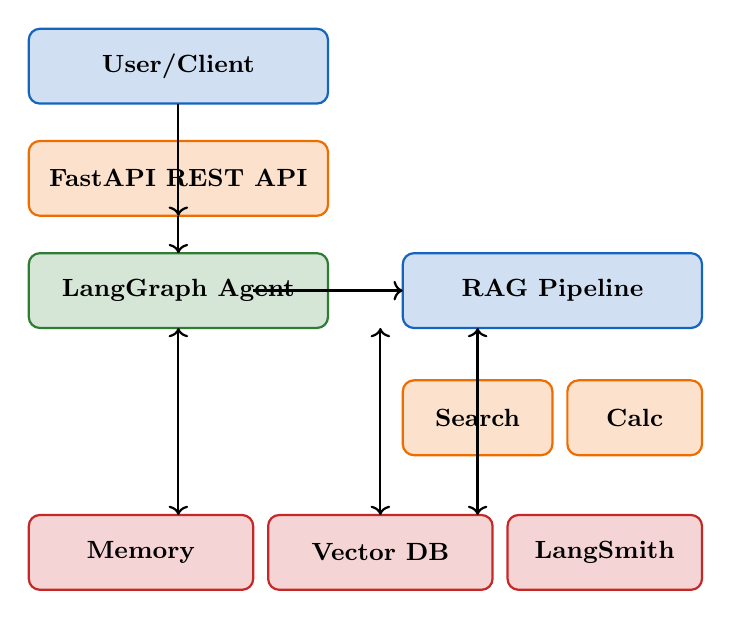
\begin{tikzpicture}[scale=0.95, every node/.style={font=\small}]
    \draw[rounded corners, fill=lcblue!20, thick, draw=lcblue] (0, 8.5) rectangle (4, 9.5);
    \node at (2, 9) {\textbf{User/Client}};

    \draw[rounded corners, fill=lcorange!20, thick, draw=lcorange] (0, 7) rectangle (4, 8);
    \node at (2, 7.5) {\textbf{FastAPI REST API}};

    \draw[rounded corners, fill=lcgreen!20, thick, draw=lcgreen] (0, 5.5) rectangle (4, 6.5);
    \node at (2, 6) {\textbf{LangGraph Agent}};

    \draw[rounded corners, fill=lcblue!20, thick, draw=lcblue] (5, 5.5) rectangle (9, 6.5);
    \node at (7, 6) {\textbf{RAG Pipeline}};

    \draw[rounded corners, fill=lcorange!20, thick, draw=lcorange] (5, 3.8) rectangle (7, 4.8);
    \node at (6, 4.3) {\textbf{Search}};

    \draw[rounded corners, fill=lcorange!20, thick, draw=lcorange] (7.2, 3.8) rectangle (9, 4.8);
    \node at (8.1, 4.3) {\textbf{Calc}};

    \draw[rounded corners, fill=lcred!20, thick, draw=lcred] (0, 2) rectangle (3, 3);
    \node at (1.5, 2.5) {\textbf{Memory}};

    \draw[rounded corners, fill=lcred!20, thick, draw=lcred] (3.2, 2) rectangle (6.2, 3);
    \node at (4.7, 2.5) {\textbf{Vector DB}};

    \draw[rounded corners, fill=lcred!20, thick, draw=lcred] (6.4, 2) rectangle (9, 3);
    \node at (7.7, 2.5) {\textbf{LangSmith}};

    \draw[->, thick] (2, 8.5) -- (2, 7);
    \draw[->, thick] (2, 7) -- (2, 6.5);
    \draw[->, thick] (3, 6) -- (5, 6);
    \draw[<->, thick] (2, 5.5) -- (2, 3);
    \draw[<->, thick] (6, 5.5) -- (6, 3);
    \draw[<->, thick] (4.7, 5.5) -- (4.7, 3);
  \end{tikzpicture}
\end{frame}

% ============================================================================
% SLIDE 4: Project Structure
% ============================================================================
\begin{frame}[fragile]
  \frametitle{Project Structure}

  \begin{lstlisting}
rag_chatbot/
  requirements.txt       -- Dependencies
  .env                   -- API keys
  src/
    ingestion.py        -- Document loading
    retriever.py        -- RAG chain
    tools.py            -- Custom tools
    agent.py            -- LangGraph agent
    memory.py           -- Conversation memory
  api/
    main.py             -- FastAPI app
  run.py                -- Entry point
  \end{lstlisting}
\end{frame}

% ============================================================================
% SLIDE 5: Dependencies
% ============================================================================
\begin{frame}[fragile]
  \frametitle{requirements.txt}

  \begin{lstlisting}
langchain>=0.1.0
langchain-openai>=0.0.1
langgraph>=0.0.1
langsmith>=0.0.1
fastapi>=0.104.0
uvicorn>=0.24.0
openai>=1.3.0
pinecone-client>=3.0.0
python-dotenv>=1.0.0
  \end{lstlisting}
\end{frame}

% ============================================================================
% SLIDE 6: Step 1 - Ingestion (Part A)
% ============================================================================
\begin{frame}[fragile]
  \frametitle{Step 1: Document Ingestion Pipeline (Part A)}

  \begin{lstlisting}
from langchain_community.document_loaders
  import PyPDFLoader
from langchain.text_splitter
  import RecursiveCharacterTextSplitter

def load_documents(doc_path):
    loader = PyPDFLoader(doc_path)
    return loader.load()

def split_documents(documents,
    chunk_size=1000):
    splitter = RecursiveCharacterTextSplitter(
        chunk_size=chunk_size,
        chunk_overlap=200,
        separators=["\n\n", "\n"])
    return splitter.split_documents(documents)
  \end{lstlisting}
\end{frame}

% ============================================================================
% SLIDE 7: Step 1 - Ingestion (Part B)
% ============================================================================
\begin{frame}[fragile]
  \frametitle{Step 1: Document Ingestion Pipeline (Part B)}

  \begin{lstlisting}
from langchain_openai import OpenAIEmbeddings
from pinecone import Pinecone

def create_vector_store(chunks):
    embeddings = OpenAIEmbeddings(
        model="text-embedding-3-small")

    pc = Pinecone(api_key=os.getenv(
        "PINECONE_API_KEY"))
    index = pc.Index("rag-chatbot-index")

    for chunk in chunks:
        embedding = embeddings.embed_query(
            chunk.page_content)
        index.upsert([(chunk.metadata["source"],
          embedding, chunk.page_content)])

    return index
  \end{lstlisting}
\end{frame}

% ============================================================================
% SLIDE 8: Step 2 - RAG Chain
% ============================================================================
\begin{frame}[fragile]
  \frametitle{Step 2: Building the Retrieval Chain}

  \begin{lstlisting}
from langchain.chains import RetrievalQA
from langchain_openai import ChatOpenAI

def create_retrieval_chain(vector_store):
    llm = ChatOpenAI(
        model="gpt-4-turbo-preview",
        temperature=0.7,
        streaming=True)

    rag_chain = RetrievalQA.from_chain_type(
        llm=llm,
        chain_type="stuff",
        retriever=vector_store.as_retriever(
            k=4))

    return rag_chain
  \end{lstlisting}
\end{frame}

% ============================================================================
% SLIDE 9: Step 3 - Tools (Part A)
% ============================================================================
\begin{frame}[fragile]
  \frametitle{Step 3: Adding Tool Capabilities (Part A)}

  \begin{lstlisting}
from langchain.tools import Tool
import requests

def search_web(query: str) -> str:
    headers = {"X-API-KEY":
        os.getenv("SERPER_API_KEY")}
    response = requests.get(
        "https://google.serper.dev/search",
        params={"q": query},
        headers=headers)
    results = response.json()
    return str(results.get("organic", []))

def calculate(expression: str) -> str:
    try:
        from sympy import sympify
        return str(sympify(expression))
    except:
        return "Invalid"
  \end{lstlisting}
\end{frame}

% ============================================================================
% SLIDE 10: Step 3 - Tools (Part B)
% ============================================================================
\begin{frame}[fragile]
  \frametitle{Step 3: Adding Tool Capabilities (Part B)}

  \begin{lstlisting}
web_search = Tool(
    name="WebSearch",
    func=search_web,
    description="Search the web")

calc_tool = Tool(
    name="Calculator",
    func=calculate,
    description="Evaluate math")

retrieval_tool = Tool(
    name="DocumentRetrieval",
    func=retrieve_from_docs,
    description="Retrieve from docs")

tools = [web_search, calc_tool,
    retrieval_tool]
  \end{lstlisting}
\end{frame}

% ============================================================================
% SLIDE 11: Step 4 - LangGraph (Part A)
% ============================================================================
\begin{frame}[fragile]
  \frametitle{Step 4: Creating Agent with LangGraph (Part A)}

  \begin{lstlisting}
from langgraph.graph import StateGraph, END
from langchain_openai import ChatOpenAI

def build_agent_graph(tools):
    def agent_node(state):
        llm = ChatOpenAI(
            model="gpt-4-turbo-preview")
        llm_with_tools = llm.bind_tools(tools)
        messages = state.get("messages", [])
        response = llm_with_tools.invoke(
            messages)
        return {"messages":
            messages + [response]}

    def should_continue(state):
        messages = state.get("messages", [])
        if not messages:
            return END
        return "tools"
  \end{lstlisting}
\end{frame}

% ============================================================================
% SLIDE 12: Step 4 - LangGraph (Part B)
% ============================================================================
\begin{frame}[fragile]
  \frametitle{Step 4: Creating Agent with LangGraph (Part B)}

  \begin{lstlisting}
    def tool_node(state):
        messages = state.get("messages", [])
        last = messages[-1] if messages else None
        if last and hasattr(last,
            "tool_calls"):
            for call in last.tool_calls:
                name = call.get("name")
                args = call.get("args")
                # Execute tool
        return {"executed": True}

    workflow = StateGraph(dict)
    workflow.add_node("agent", agent_node)
    workflow.add_node("tools", tool_node)
    workflow.add_edge("tools", "agent")
    workflow.add_conditional_edges(
        "agent", should_continue)
    workflow.set_entry_point("agent")
    return workflow.compile()
  \end{lstlisting}
\end{frame}

% ============================================================================
% SLIDE 13: Step 5 - Memory
% ============================================================================
\begin{frame}[fragile]
  \frametitle{Step 5: Adding Conversation Memory}

  \begin{lstlisting}
from langgraph.checkpoint.sqlite
  import SqliteSaver
import sqlite3

def setup_memory(db_path="chat_history.db"):
    conn = sqlite3.connect(db_path)
    cursor = conn.cursor()
    cursor.execute('''CREATE TABLE IF NOT
      EXISTS messages (id INTEGER PRIMARY
      KEY, session_id TEXT, role TEXT,
      content TEXT, timestamp DATETIME)''')
    conn.commit()
    return SqliteSaver(connection=conn)

def save_message(session_id, role, content):
    conn = sqlite3.connect("chat_history.db")
    cursor = conn.cursor()
    cursor.execute('''INSERT INTO messages
      (session_id, role, content)
      VALUES (?, ?, ?)''',
      (session_id, role, content))
    conn.commit()
  \end{lstlisting}
\end{frame}

% ============================================================================
% SLIDE 14: Step 6 - Streaming
% ============================================================================
\begin{frame}[fragile]
  \frametitle{Step 6: Adding Streaming Support}

  \begin{lstlisting}
from typing import AsyncIterator

async def stream_agent_response(
    executor, user_input, session_id
) -> AsyncIterator[str]:
    history = load_conversation(session_id)
    messages = []
    for m in history:
        if m.get("role") == "user":
            messages.append(
              HumanMessage(m.get("content")))
        else:
            messages.append(
              AIMessage(m.get("content")))

    messages.append(HumanMessage(user_input))
    async for event in
        executor.astream_events(messages):
        if "stream" in event:
            yield event
  \end{lstlisting}
\end{frame}

% ============================================================================
% SLIDE 15: Step 7 - LangSmith
% ============================================================================
\begin{frame}[fragile]
  \frametitle{Step 7: Adding LangSmith Tracing}

  \begin{lstlisting}
import os

def setup_langsmith():
    os.environ["LANGCHAIN_TRACING_V2"] = "true"
    os.environ["LANGCHAIN_PROJECT"] =
      "rag-chatbot"
    os.environ["LANGCHAIN_ENDPOINT"] =
      "https://api.smith.langchain.com"
    os.environ["LANGCHAIN_API_KEY"] =
      os.getenv("LANGSMITH_API_KEY")

# Every agent run is automatically traced
# Traces include:
#   - Full conversation flow
#   - Tool invocations
#   - Token counts and latency
#   - Errors and exceptions
  \end{lstlisting}

  \begin{tipbox}[Benefits]
    \small Monitor costs, debug flows, A/B test prompts
  \end{tipbox}
\end{frame}

% ============================================================================
% SLIDE 16: Step 8 - API (Part A)
% ============================================================================
\begin{frame}[fragile]
  \frametitle{Step 8: Building the API Layer (Part A)}

  \begin{lstlisting}
from fastapi import FastAPI
from pydantic import BaseModel

app = FastAPI(title="RAG Chatbot")

class ChatMessage(BaseModel):
    session_id: str
    user_input: str

class ChatResponse(BaseModel):
    session_id: str
    response: str

@app.post("/chat")
async def chat(message: ChatMessage):
    history = load_conversation(
        message.session_id)
    result = await executor.ainvoke(history)
    save_message(message.session_id,
      "assistant", result)
    return ChatResponse(
        session_id=message.session_id,
        response=result)
  \end{lstlisting}
\end{frame}

% ============================================================================
% SLIDE 17: Step 8 - API (Part B)
% ============================================================================
\begin{frame}[fragile]
  \frametitle{Step 8: Building the API Layer (Part B)}

  \begin{lstlisting}
from fastapi.responses \
  import StreamingResponse

@app.post("/chat/stream")
async def chat_stream(message: ChatMessage):
    async def stream_generator():
        try:
            async for token in \
                stream_agent_response(executor,
                message.user_input,
                message.session_id):
                yield "data: " + token + "\n\n"
        except Exception as e:
            yield "data: ERROR\n\n"

    return StreamingResponse(
        stream_generator(),
        media_type="text/event-stream")

@app.get("/history/{session_id}")
async def get_history(session_id: str):
    return load_conversation(session_id)
  \end{lstlisting}
\end{frame}

% ============================================================================
% SLIDE 18: Step 9 - Error Handling
% ============================================================================
\begin{frame}[fragile]
  \frametitle{Step 9: Error Handling and Fallbacks}

  \begin{lstlisting}
import logging
from functools import wraps

logger = logging.getLogger(__name__)

def with_fallback(fallback_response):
    def decorator(func):
        @wraps(func)
        async def wrapper(*args, **kwargs):
            try:
                return await func(
                    *args, **kwargs)
            except Exception as e:
                logger.error(str(e))
                return fallback_response
        return wrapper
    return decorator

@with_fallback("Could not process request")
async def agent_call(user_input):
    return await executor.ainvoke(
        {"input": user_input})
  \end{lstlisting}
\end{frame}

% ============================================================================
% SLIDE 19: Step 10 - Testing
% ============================================================================
\begin{frame}[fragile]
  \frametitle{Step 10: Testing the System}

  \begin{lstlisting}
import pytest
from langchain.schema import HumanMessage

@pytest.mark.asyncio
async def test_agent_with_tool():
    executor = build_agent_executor()
    msg = HumanMessage(
        content="What is 15 * 23?")
    result = await executor.ainvoke(
        {"messages": [msg]})
    assert "345" in str(result)

@pytest.mark.asyncio
async def test_document_retrieval():
    executor = build_agent_executor()
    msg = HumanMessage(
        content="What does section 3 say?")
    result = await executor.ainvoke(
        {"messages": [msg]})
    assert len(result) > 0
  \end{lstlisting}
\end{frame}

% ============================================================================
% SLIDE 20: Data Flow
% ============================================================================
\begin{frame}
  \frametitle{Complete Data Flow}

  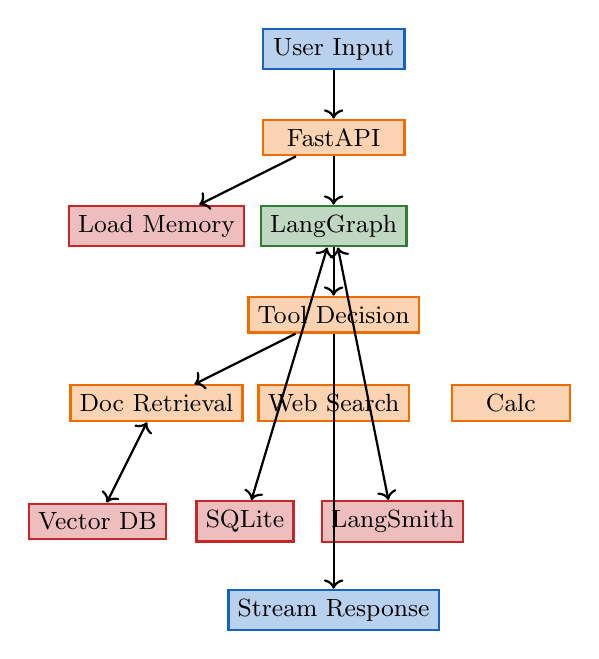
\begin{tikzpicture}[scale=0.75, every node/.style={font=\small}]
    \node[rectangle, fill=lcblue!30, draw=lcblue, thick, minimum width=1.8cm] (user) at (0, 10) {User Input};
    \node[rectangle, fill=lcorange!30, draw=lcorange, thick, minimum width=1.8cm] (api) at (0, 8.5) {FastAPI};
    \node[rectangle, fill=lcred!30, draw=lcred, thick, minimum width=1.8cm] (history) at (-3, 7) {Load Memory};
    \node[rectangle, fill=lcgreen!30, draw=lcgreen, thick, minimum width=1.8cm] (agent) at (0, 7) {LangGraph};
    \node[rectangle, fill=lcorange!30, draw=lcorange, thick, minimum width=1.8cm] (decision) at (0, 5.5) {Tool Decision};
    \node[rectangle, fill=lcorange!30, draw=lcorange, thick, minimum width=1.5cm] (docret) at (-3, 4) {Doc Retrieval};
    \node[rectangle, fill=lcorange!30, draw=lcorange, thick, minimum width=1.5cm] (websearch) at (0, 4) {Web Search};
    \node[rectangle, fill=lcorange!30, draw=lcorange, thick, minimum width=1.5cm] (calc) at (3, 4) {Calc};
    \node[rectangle, fill=lcred!30, draw=lcred, thick, minimum width=1.2cm] (vecdb) at (-4, 2) {Vector DB};
    \node[rectangle, fill=lcred!30, draw=lcred, thick, minimum width=1.2cm] (sql) at (-1.5, 2) {SQLite};
    \node[rectangle, fill=lcred!30, draw=lcred, thick, minimum width=1.2cm] (trace) at (1, 2) {LangSmith};
    \node[rectangle, fill=lcblue!30, draw=lcblue, thick, minimum width=1.8cm] (response) at (0, 0.5) {Stream Response};

    \draw[->, thick] (user) -- (api);
    \draw[->, thick] (api) -- (history);
    \draw[->, thick] (api) -- (agent);
    \draw[->, thick] (agent) -- (decision);
    \draw[->, thick] (decision) -- (docret);
    \draw[<->, thick] (docret) -- (vecdb);
    \draw[<->, thick] (agent) -- (sql);
    \draw[<->, thick] (agent) -- (trace);
    \draw[->, thick] (decision) -- (response);
  \end{tikzpicture}
\end{frame}

% ============================================================================
% SLIDE 21: Entry Point
% ============================================================================
\begin{frame}[fragile]
  \frametitle{Entry Point: run.py}

  \begin{lstlisting}
import asyncio
from dotenv import load_dotenv

async def main():
    load_dotenv()
    setup_langsmith()
    setup_memory()

    print("Indexing documents...")
    vector_store = ingest_all(
        "./data/documents")

    print("Building agent...")
    agent = build_agent_executor(
        vector_store)

    print("Starting API...")
    import uvicorn
    uvicorn.run("api.main:app",
      host="0.0.0.0", port=8000)

if __name__ == "__main__":
    asyncio.run(main())
  \end{lstlisting}
\end{frame}

% ============================================================================
% SLIDE 22: Running
% ============================================================================
\begin{frame}[fragile]
  \frametitle{Running the Application}

  \begin{conceptbox}[Step 1: Setup]
    \tiny
    \begin{lstlisting}
python -m venv venv
source venv/bin/activate
pip install -r requirements.txt
    \end{lstlisting}
  \end{conceptbox}

  \begin{conceptbox}[Step 2: Configure]
    \tiny
    \begin{lstlisting}
OPENAI_API_KEY=sk-...
PINECONE_API_KEY=...
LANGSMITH_API_KEY=...
    \end{lstlisting}
  \end{conceptbox}

  \begin{conceptbox}[Step 3: Run]
    \tiny
    \begin{lstlisting}
python run.py
    \end{lstlisting}
  \end{conceptbox}
\end{frame}

% ============================================================================
% SLIDE 23: Testing API
% ============================================================================
\begin{frame}[fragile]
  \frametitle{Testing the API}

  \begin{codebox}[Using curl]
    \tiny
    \begin{lstlisting}
curl -X POST http://localhost:8000/chat \
  -H "Content-Type: application/json" \
  -d '{"session_id":"user123",
       "user_input":"What is section 3?"}'
    \end{lstlisting}
  \end{codebox}

  \begin{codebox}[Using Python]
    \tiny
    \begin{lstlisting}
import requests
response = requests.post(
    "http://localhost:8000/chat",
    json={"session_id": "user123",
          "user_input": "Calculate 42*17"})
print(response.json())
    \end{lstlisting}
  \end{codebox}
\end{frame}

% ============================================================================
% SLIDE 24: Components Recap
% ============================================================================
\begin{frame}
  \frametitle{Recap: What We Used From Each Section}

  \begin{tiny}
    \begin{tabular}{|l|l|l|}
      \toprule
      \textbf{Task} & \textbf{Component} & \textbf{Section} \\
      \midrule
      Load PDFs & PyPDFLoader & 1 \\
      Split text & RecursiveCharacterTextSplitter & 1 \\
      Embeddings & OpenAIEmbeddings & 3 \\
      Vector search & Pinecone & 3 \\
      Chains & RetrievalQA & 2 \\
      Memory & SqliteSaver & 4 \\
      Tools & Tool class & 5 \\
      Agent & StateGraph & 7 \\
      Streaming & async iterators & 8 \\
      API & FastAPI & 9 \\
      Tracing & LangSmith & 10 \\
      \bottomrule
    \end{tabular}
  \end{tiny}
\end{frame}

% ============================================================================
% SLIDE 25: Key Lessons
% ============================================================================
\begin{frame}
  \frametitle{Key Lessons: Building Production Systems}

  \begin{itemize}
    \item \textbf{Start simple:} Begin with basic RAG, add agents later
    \item \textbf{Memory matters:} Persistent history is essential
    \item \textbf{Streaming improves UX:} Real-time feedback matters
    \item \textbf{Observability is critical:} LangSmith reveals bottlenecks
    \item \textbf{Tool selection is hard:} Agents need clear descriptions
    \item \textbf{Error handling required:} Plan for API/retrieval failures
    \item \textbf{Testing essential:} Mock tools for fast iteration
    \item \textbf{Monitor costs:} Track token usage carefully
    \item \textbf{Security first:} Never commit API keys
  \end{itemize}
\end{frame}

% ============================================================================
% SLIDE 26: Enhancement Ideas
% ============================================================================
\begin{frame}
  \frametitle{Enhancement Ideas}

  \begin{columns}[T]
    \column{0.5\textwidth}
    \textbf{Capability}
    \begin{itemize}
      \item Multi-turn reasoning
      \item Document citations
      \item Clarification questions
      \item Follow-up suggestions
    \end{itemize}

    \column{0.5\textwidth}
    \textbf{System}
    \begin{itemize}
      \item Prompt optimization
      \item Fine-tuning on Q\&A
      \item Rate limiting
      \item Web UI
    \end{itemize}
  \end{columns}

  \begin{columns}[T]
    \column{0.5\textwidth}
    \textbf{Integration}
    \begin{itemize}
      \item Slack/Teams bot
      \item Webhooks
      \item Database integration
      \item File upload
    \end{itemize}

    \column{0.5\textwidth}
    \textbf{Monitoring}
    \begin{itemize}
      \item A/B testing
      \item User satisfaction
      \item Cost tracking
      \item Alerts
    \end{itemize}
  \end{columns}
\end{frame}

% ============================================================================
% SLIDE 27: Multi-Agent Pattern
% ============================================================================
\begin{frame}[fragile]
  \frametitle{Advanced: Multi-Agent Collaboration}

  \begin{lstlisting}
supervisor_prompt = "You supervise agents"

def supervisor_node(state):
    messages = state.get("messages", [])
    llm = ChatOpenAI(
        model="gpt-4-turbo-preview")
    route = llm.invoke(messages)
    return {"next_agent": route.next}

workflow = StateGraph(dict)
workflow.add_node("supervisor",
    supervisor_node)
workflow.add_node("retrieval_agent",
    retrieval_agent)
workflow.add_node("web_agent", web_agent)
workflow.add_conditional_edges(
    "supervisor",
    lambda x: x.get("next_agent", "end"))
  \end{lstlisting}
\end{frame}

% ============================================================================
% SLIDE 28: Custom Memory
% ============================================================================
\begin{frame}[fragile]
  \frametitle{Advanced: Custom Memory Types}

  \begin{lstlisting}
class ContextualMemory:
    def __init__(self, max_tokens=2000):
        self.messages = []
        self.max_tokens = max_tokens

    def add(self, message):
        self.messages.append(message)
        self._prune_old_messages()

    def _prune_old_messages(self):
        embeddings = OpenAIEmbeddings()
        # Score by relevance
        # Keep high-scoring

    def get_relevant(self, query):
        # Return relevant messages
        pass
  \end{lstlisting}
\end{frame}

% ============================================================================
% SLIDE 29: Dynamic Tools
% ============================================================================
\begin{frame}[fragile]
  \frametitle{Advanced: Dynamic Tool Selection}

  \begin{lstlisting}
def select_best_tools(query):
    embeddings = OpenAIEmbeddings()
    query_emb = embeddings.embed_query(query)

    tool_scores = []
    for tool in all_tools:
        desc_emb = embeddings.embed_query(
            tool.description)
        score = cosine_similarity(
            query_emb, desc_emb)
        tool_scores.append((tool, score))

    return [t for t, s in tool_scores
            if s > 0.7]

def smart_agent(state):
    messages = state.get("messages", [])
    query = messages[-1].content if messages
    tools = select_best_tools(query)
    return ChatOpenAI().bind_tools(
        tools).invoke(messages)
  \end{lstlisting}
\end{frame}

% ============================================================================
% SLIDE 30: Deployment
% ============================================================================
\begin{frame}
  \frametitle{Deployment Patterns}

  \begin{columns}[T]
    \column{0.5\textwidth}
    \textbf{Development}
    \begin{itemize}
      \item Local SQLite
      \item Mock LLM
      \item Fast iteration
    \end{itemize}

    \column{0.5\textwidth}
    \textbf{Production}
    \begin{itemize}
      \item PostgreSQL
      \item Real API
      \item Rate limiting
    \end{itemize}
  \end{columns}

  \begin{columns}[T]
    \column{0.5\textwidth}
    \textbf{Docker}
    \begin{itemize}
      \item Container-based
      \item Kubernetes
      \item Isolation
    \end{itemize}

    \column{0.5\textwidth}
    \textbf{Serverless}
    \begin{itemize}
      \item AWS Lambda
      \item Auto-scaling
      \item Pay-per-call
    \end{itemize}
  \end{columns}
\end{frame}

% ============================================================================
% SLIDE 31: Docker
% ============================================================================
\begin{frame}[fragile]
  \frametitle{Docker Deployment}

  \begin{lstlisting}
FROM python:3.11-slim
WORKDIR /app
COPY requirements.txt .
RUN pip install --no-cache-dir \
  -r requirements.txt
COPY . .
ENV PYTHONUNBUFFERED=1
CMD ["python", "run.py"]
  \end{lstlisting}

  \begin{lstlisting}
version: '3'
services:
  chatbot:
    build: .
    ports:
      - "8000:8000"
    environment:
      OPENAI_API_KEY: APIkey
      PINECONE_API_KEY: APIkey
  \end{lstlisting}
\end{frame}

% ============================================================================
% SLIDE 32: Monitoring
% ============================================================================
\begin{frame}[fragile]
  \frametitle{Monitoring and Logging}

  \begin{lstlisting}
import logging

logging.basicConfig(
    level=logging.INFO,
    format="%(asctime)s %(message)s",
    handlers=[
        logging.FileHandler("chatbot.log"),
        logging.StreamHandler()
    ])

logger = logging.getLogger(__name__)

def agent_node(state):
    msgs = state.get("messages", [])
    logger.info(f"Processing {len(msgs)} msgs")
    try:
        response = llm.invoke(msgs)
        logger.info(f"Response: {len(response)}")
        return response
    except Exception as e:
        logger.error(f"Error: {e}")
        raise
  \end{lstlisting}
\end{frame}

% ============================================================================
% SLIDE 33: Cost Optimization
% ============================================================================
\begin{frame}
  \frametitle{Cost Optimization Strategies}

  \begin{itemize}
    \item Use smaller models for simple tasks
    \item Batch requests to amortize API calls
    \item Cache embeddings and pre-compute
    \item Limit retriever scope with ranking
    \item Monitor token usage per conversation
    \item Use function calling efficiently
    \item Implement request quotas
    \item A/B test prompts for cost/quality
  \end{itemize}

  \begin{tipbox}[Cost Tracking]
    \small Log token usage per request and aggregate in LangSmith.
  \end{tipbox}
\end{frame}

% ============================================================================
% SLIDE 34: Security
% ============================================================================
\begin{frame}
  \frametitle{Security Best Practices}

  \begin{itemize}
    \item \textbf{Environment variables:} Never hardcode keys
    \item \textbf{Input validation:} Sanitize user queries
    \item \textbf{Rate limiting:} Prevent abuse
    \item \textbf{Authentication:} Require API tokens
    \item \textbf{HTTPS only:} Encrypt in transit
    \item \textbf{Data retention:} Delete old conversations
    \item \textbf{Audit logs:} Track access
    \item \textbf{Isolation:} Containers with minimal privileges
  \end{itemize}
\end{frame}

% ============================================================================
% SLIDE 35: Performance
% ============================================================================
\begin{frame}
  \frametitle{Performance Tuning}

  \begin{columns}[T]
    \column{0.5\textwidth}
    \textbf{Latency}
    \begin{itemize}
      \item Async/await for I/O
      \item Parallel tool execution
      \item Cache frequent queries
      \item Connection pooling
    \end{itemize}

    \column{0.5\textwidth}
    \textbf{Throughput}
    \begin{itemize}
      \item Load balancing
      \item Worker processes
      \item Horizontal scaling
      \item Queue-based architecture
    \end{itemize}
  \end{columns}

  \begin{tipbox}[Profiling]
    \small Use cProfile and LangSmith traces to find bottlenecks.
  \end{tipbox}
\end{frame}

% ============================================================================
% SLIDE 36: Debugging
% ============================================================================
\begin{frame}
  \frametitle{Debugging Common Issues}

  \begin{tabular}{|l|l|}
    \toprule
    \textbf{Issue} & \textbf{Solution} \\
    \midrule
    Agent won't use tools & Check descriptions \\
    Poor retrieval & Tune chunk size \\
    Tool errors & Add error handling \\
    Memory bloat & Implement pruning \\
    Slow responses & Profile with LangSmith \\
    Inconsistent outputs & Tune temperature \\
    Token limit exceeded & Summarize \\
    \bottomrule
  \end{tabular}
\end{frame}

% ============================================================================
% SLIDE 37: Self-Check (1)
% ============================================================================
\begin{frame}
  \frametitle{Self-Check Questions (1/2)}

  \begin{enumerate}
    \item What are the three RAG components and why each matters?
    \vspace{0.3cm}
    \item How does StateGraph differ from a simple chain?
    \vspace{0.3cm}
    \item What is checkpointing in memory?
    \vspace{0.3cm}
    \item How to implement streaming in FastAPI?
    \vspace{0.3cm}
  \end{enumerate}
\end{frame}

% ============================================================================
% SLIDE 38: Self-Check (2)
% ============================================================================
\begin{frame}
  \frametitle{Self-Check Questions (2/2)}

  \begin{enumerate}
    \setcounter{enumi}{4}
    \item Why is dynamic tool selection via embeddings better?
    \vspace{0.3cm}
    \item Three ways to optimize cost in production RAG?
    \vspace{0.3cm}
    \item Debug an agent that never uses web search?
    \vspace{0.3cm}
    \item What to add for enterprise use?
    \vspace{0.3cm}
  \end{enumerate}
\end{frame}

% ============================================================================
% SLIDE 39: What's Next
% ============================================================================
\begin{frame}
  \frametitle{What's Next? Advanced Topics}

  \begin{itemize}
    \item \textbf{Fine-tuning:} Adapt to your domain
    \item \textbf{Multi-modal RAG:} Images, videos, tables
    \item \textbf{Graph RAG:} Knowledge graphs
    \item \textbf{Recursive summarization:} Large documents
    \item \textbf{Adversarial robustness:} Handle jailbreaks
    \item \textbf{Custom evaluation:} Correctness checks
    \item \textbf{Federated learning:} Distributed data
    \item \textbf{Real-time updates:} Zero-downtime deployment
  \end{itemize}
\end{frame}

% ============================================================================
% SLIDE 40: Summary
% ============================================================================
\begin{frame}
  \frametitle{Summary: Key Takeaways}

  \begin{conceptbox}[The Complete System]
    A production RAG chatbot requires:
    \begin{itemize}
      \item Ingestion: Load, split, embed documents
      \item Retrieval: Index and retrieve vectors
      \item Agents: Select and use tools
      \item Memory: Persist context
      \item APIs: Expose via REST with streaming
      \item Observability: Trace every call
      \item Production: Deploy, scale, monitor
    \end{itemize}
  \end{conceptbox}

  \begin{warningbox}[Remember]
    Start simple (basic RAG), validate, then add complexity. Every feature has a cost.
  \end{warningbox}
\end{frame}

% ============================================================================
% SLIDE 41: Resources
% ============================================================================
\begin{frame}
  \frametitle{Resources and References}

  \begin{itemize}
    \item \textbf{LangChain:} https://python.langchain.com
    \item \textbf{LangGraph:} https://langchain-ai.github.io/langgraph
    \item \textbf{LangSmith:} https://docs.smith.langchain.com
    \item \textbf{OpenAI API:} https://platform.openai.com/docs
    \item \textbf{Pinecone:} https://docs.pinecone.io
    \item \textbf{FastAPI:} https://fastapi.tiangolo.com
    \item \textbf{Examples:} LangChain GitHub
  \end{itemize}
\end{frame}

% ============================================================================
% SLIDE 42: Closing
% ============================================================================
\begin{frame}
  \frametitle{You Now Know...}

  \begin{center}
    {\Large \textbf{How to build a production-grade}} \\
    \vspace{0.3cm}
    {\Large \textbf{LangChain application from scratch}}
    \vspace{0.6cm}

    \begin{itemize}
      \item Document ingestion at scale
      \item Retrieval-augmented generation
      \item Multi-tool agent orchestration
      \item Persistent memory
      \item Real-time streaming
      \item Full observability
      \item Deployment and monitoring
    \end{itemize}

    \vspace{0.6cm}
    {\small The next step: Build your own and iterate!}
  \end{center}
\end{frame}

% ============================================================================
% SLIDE 43: Thank You
% ============================================================================
\begin{frame}[plain]
  \begin{center}
    \vspace{2cm}
    {\Huge Thank you!}
    \vspace{0.8cm}

    {\Large Questions?}
    \vspace{0.8cm}

    Let's discuss implementation, architecture, or your project ideas.

    \vspace{1.2cm}
    \docref{LangChain v1.2.x Documentation}
  \end{center}
\end{frame}

\end{document}
